%%%%%%%%%%%%%%%%%%%%%%%%%%%%%%%%%%%%%%%%%%%%%%%%%%%
%
%  New template code for TAMU Theses and Dissertations starting Fall 2012.  
%  For more info about this template or the 
%  TAMU LaTeX User's Group, see http://www.howdy.me/.
%
%  Author: Wendy Lynn Turner 
%	 Version 1.0 
%  Last updated 8/5/2012
%
%%%%%%%%%%%%%%%%%%%%%%%%%%%%%%%%%%%%%%%%%%%%%%%%%%%
%%%                           APPENDIX - Chapter 3
%%%%%%%%%%%%%%%%%%%%%%%%%%%%%%%%%%%%%%%%%%%%%%%%%%%

\phantomsection
\chapter{\uppercase{Addendum to Section \ref{sec::BF}}}
\label{sec::appendix_BF}

%%%%%%%%%%%%%%%%%%%%%%%%%%%%%%%%%%%%%%%%%%%%%%%%%%%
%%%   Section - Limits of the Linear Polygonal Basis Functions
\section{Limits of the Linear Polygonal Basis Functions}
\label{sec::appendix_BF_Limits}

As it was stated in Section \ref{sec::BF_2DLinear}, the Wachspress, mean value, and maximum entropy coordinates are all undefined on the boundary of the polygonal element. 

\begin{figure}[hbt]
\centering
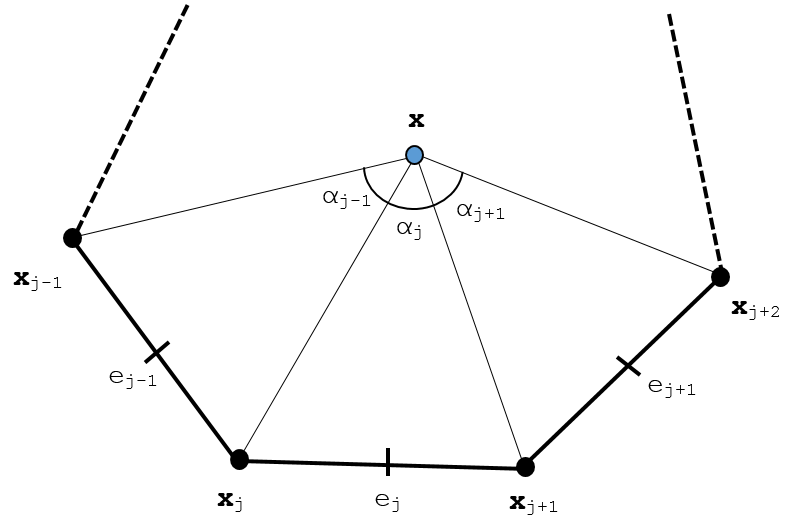
\includegraphics[width=0.65\textwidth]{figures/appendices/ref_polygon.png}
\caption{Arbitrary polygon with geometric properties used for 2D basis function generation.}
\label{fig::App_BF_2D_ref_polygon}
\end{figure}

%%%%%%%%%%%%%%%%%%%%%%%%%%%%%%%%%%%%%%%%%%%%%%%%%%%
%%%  Sub Section - Wachspress Limits
\subsection{Limits of the Wachspress Coordinates}
\label{sec::appendix_BF_Limits_Wachspress}

\begin{equation}
\label{eq::App_BF_WachBF}
\lambda_i^{W} (\vec{x}) = \frac{w_i^W  (\vec{x}) }{\sum_j w_j^W  (\vec{x}) }
\end{equation}

%%%%%%%%%%%%%%%%%%%%%%%%%%%%%%%%%%%%%%%%%%%%%%%%%%%
%%%  Sub Section - MV Limits
\subsection{Limits of the Mean Value Coordinates}
\label{sec::appendix_BF_Limits_MV}

\begin{equation}
\label{eq::App_BF_MVBF}
\lambda_i^{MV} (\vec{x}) = \frac{w_i^{MV}  (\vec{x}) }{\sum_j w_j^{MV}  (\vec{x}) }
\end{equation}

%%%%%%%%%%%%%%%%%%%%%%%%%%%%%%%%%%%%%%%%%%%%%%%%%%%
%%%  Sub Section - ME Limits
\subsection{Limits of the Maximum Entropy Coordinates}
\label{sec::appendix_BF_Limits_ME}


\begin{equation}
\label{eq::App_BF_MEBF}
\lambda_i^{ME} (\vec{x}) = \frac{w_i^{ME}  (\vec{x}) }{\sum_j w_j^{ME}  (\vec{x}) }
\end{equation}